\chapter{Copula}
\label{ch-copula}

This chapter is based 
on Refs.\cite{wiki-copula}
and \cite{copula-bo}.

A copula in architecture is a domed roof. Here we will discuss a copula in Statistics.
Copulas are probably called this in Statistics
because their probability density resembles a dome when their domain is 
the real plane $\RR^2$.
Furthermore,
the word \enquote{copula} means
\enquote{connector} or \enquote{coupler} in Latin,
and both,
the copula in Architecture
and the one in Statistics,
connect the sides (or marginals in the
Statistics case) of a geometrical 
shape.

Let $x= [x_i]_{i=1}^n\in\RR$ be an $n$ 
dimensional column vector.
Given a probability
distribution (actually, a density) $P(x)$,
we will refer to $P(\rvx_i=x_i)$ for all $i$
as its {\bf marginals}
and to $P(\rvx_i\leq x_i)$ for all $i$
as its {\bf cumulative marginals} or {\bf c-marginals} for short.
This is normally referred
to as the {\bf CDF (cumulative
distribution function)} of $\rvx_i$.

Suppose you know the marginals $P(x_i)$ 
of  $P(x)$,
but you don't know $P(x)$
itself. There are
infinitely many
possible $P(x)$'s
with those marginals.
Informally
speaking,
a {\bf copula} is one of those
$P(x)$, a smooth one.
The dimension $n$ of
the domain of the copula,
is referred to as the
{\bf copula dimension}.
See Figs. \ref{fig-copula1}
and \ref{fig-copula2}
for examples of 2-dimensional copulas.

\begin{figure}[!h]
\begin{floatrow}
 \ffigbox{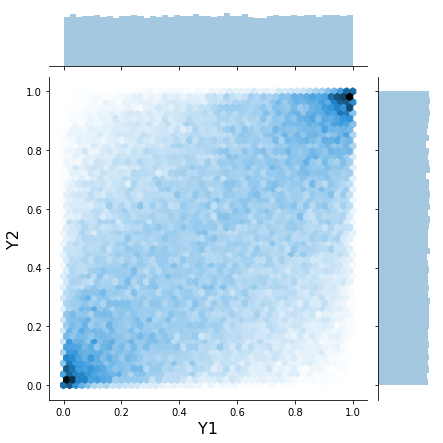
\includegraphics[width=2.5in]
 {copula/copula1.png}}
 {\caption{Contour plot of a 2-dimensional copula
 with uniform marginals}
 \label{fig-copula1}}
 \ffigbox{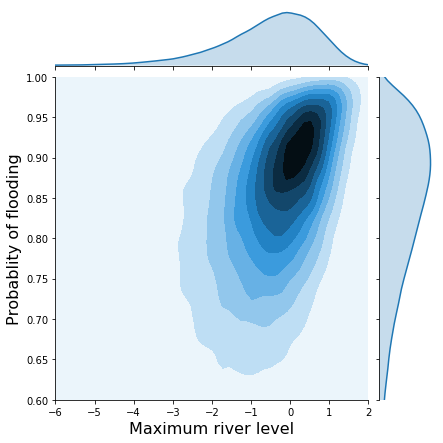
\includegraphics[width=2.5in]
 {copula/copula2.png}}
 {\caption{Contour plot of a 2-dimensional copula
 with skewed bell-shaped marginals.}
 \label{fig-copula2}}
\end{floatrow}
\end{figure}





\begin{figure}[h!]
$$
\xymatrix{
u_1
&x_1\ar[l]_{\Phi_{\rvx_1}}\ar[dd]
\\
\\
u_2
&x_2\ar[l]_{\Phi_{\rvx_2}}
}
\xymatrix{P(x_1)
\\
&=P(u, x)=&}
\xymatrix{P(u_1)
\\}
\xymatrix{
u_1\ar[dd]\ar[r]_{\Phi_{\rvx_1}^{-1}}
&x_1
\\
\\
u_2\ar[r]_{\Phi_{\rvx_2}^{-1}}
&x_2
}
$$
\caption{Graphical representation
of Eq.(\ref{eq-copula-li-density-form}) for $n=2$.
$\Phi_{
\rvx_i}(x_i) = P(\rvx_i\leq x_i)$
is the CDF of $\rvx_i$,
and we define
$u_i = \Phi_{\rvx_i}(x_i)$}
\label{fig-copula-li-bnet}
\end{figure}

Let $x= [x_i]_{i=1}^n\in\RR^n$
and  $u= [u_i]_{i=1}^n\in\RR^n$ be $n$ 
dimensional column vectors.
Henceforth,  will denote the c-marginals 
of $\rvx_i$ by $\Phi_{\rvx_i}$

\beq
\Phi_{\rvx_i}(x_i)
=
P(\rvx_i\leq x_i)
\eeq
and 
the generalization
of this map 
to vector arguments by $\Phi_\rvx$:


\beq
x=
\left[
\begin{array}{c}
x_1
\\
x_2
\\
\cdots
\\
x_n
\end{array}
\right]
\;,\quad
\Phi_{\rvx}(x)=
\left[
\begin{array}{c}
\Phi_{\rvx_1}(x_1)
\\
\Phi_{\rvx_2}(x_2)
\\
\cdots
\\
\Phi_{\rvx_n}(x_n)
\end{array}
\right]
\eeq

More precisely,
a copula in Statistics is 
defined as follows.
A
{\bf copula density}  is a probability density $P(u)$
such that (see Fig.\ref{fig-copula-li-bnet})

\beq
\underbrace{P(u|x)}_
{\prod_{i=1}^n \delta\left(
u_i-\Phi_{\rvx_i}(x_i)
\right)}
P(x)
= P(u, x)=
\underbrace{P(x|u)}_
{\prod_{i=1}^n \delta
\left(x_i-\Phi^{-1}_
{\rvx_i}(u_i)\right)}P(u)
\eeq

\beq
\boxed{
P(\rvx=x)=\left[
\underbrace{
P(\rvu = u)
}_{\text{copula density}}
\right]_{
u =\underbrace
{\Phi_{\rvx}(x)}_{\text{c-marginals}}
}}
\label{eq-copula-li-density-form}
\eeq
A {\bf copula} $C(u)$ is defined as the  
CDF
of its copula density.

\beqa
C(u) &=& \prod_{i=1}^n
\left\{
\int_{-\infty}^{u_i}du_i'
\right\}P(\rvu=u')
\\
&=&
\underbrace{
P( \forall i:\rvu_i\leq u_i)}_
{\eqdef P(\rvu\leq u)}
\label{eq-copula-p-u-leq}
\eeqa

\beq
\partial_{u_1}
\partial_{u_2}
\ldots \partial_{u_n}
C(u) = P(u)
\eeq

There are copulas
that are well-defined 
by Eq.(\ref{eq-copula-p-u-leq}), but
not differentiable, so, 
technically, without smoothing,
their 
copula density does not exist.
For this reason,
if possible, it is always
best and most general to
state copula results in
terms of CDFs,
instead of probability densities.
For example, the boxed
Eq.(\ref{eq-copula-li-density-form})
stated in terms of CDFs, is

\beq
\boxed{
P( \rvx\leq x)=
\left[
\underbrace{
P(\rvu\leq u)
}_{\text{copula}}
\right]_{
u =
\underbrace{
\Phi_{\rvx}(x)
}_
{\text{c-marginals}}
}
}
\label{eq-copula-li-cumul-form}
\eeq

\begin{claim} $\rvu_i = \Phi_{\rvx_i}(\rvx_i)$
implies that the marginal
$P(u_i)=1$ is a uniform distribution on $[0,1]$.
\end{claim}
\proof
\beq
\rvu_i = \Phi_{\rvx_i}(\rvx_i)
=
P(\rvx_i\leq \rvx_i)=1
\eeq
If that doesn't convince you, here is another 
proof.

\beqa
P(\rvu_i\leq u_i)
&=&
P(\Phi_{\rvx_i}(\rvx_i)\leq u_i)
\\
&=&
P(\rvx_i\leq \Phi_{\rvx_i}^{-1}(u_i))
\\
&=&
\Phi_{\rvx_i}\left(
\Phi_{\rvx_i}^{-1}(u_i)
\right)
\\
&=&
u_i
\eeqa
Hence,

\beqa
P(\rvu_i=u_i)&=&
\pder{}{u_i}\int_{-\infty}^{u_i}
du'_i \; P(\rvu_i=u'_i)
\\
&=&
\pder{P(\rvu_i\leq u_i)}{u_i}
\\ &=& 1
\eeqa
\qed

\section{Examples}
In the following examples, $n=2$,
and we sometimes substitute
$(u_1, u_2)=(u,v)$,
$(x_1, x_2)=(x,y)$.

\begin{enumerate}
\item {\bf $\rvx_1$ and $\rvx_2$ are independent}

If $\rvx_1$ and $\rvx_2$ are independent,
$\rvu_1$ and $\rvu_2$ are too. Hence,

\beqa
C(u_1, u_2)
&=& P(\rvu_1\leq u_1, \rvu_2\leq u_2)
\\
&=&
P(\rvu_1\leq u_1)P(\rvu_2\leq u_2)
\\
&=&
u_1 u_2
\eeqa

\beq
C(\Phi_\rvx(x))=
\Phi_{\rvx_1}(x_1)
\Phi_{\rvx_2}(x_2)
\eeq

\beq
\partial_{x_1}\partial_{x_2}C(\Phi_\rvx(x))=
\partial_{x_1}\partial_{x_2}
\Phi_{\rvx_1}(x_1)
\Phi_{\rvx_2}(x_2)
\eeq

\beq
P(x)=P(x_1)P(x_2)
\eeq

\item {\bf $\rvx_2=\alp \rvx_2$ 
for some $\alp>0$}

If $\rvx_2 = \alp \rvx_1$
for some parameter $\alp>0$,
then

\beqa
u_1
&=&
\Phi_{\rvx_1}(x_1)
\\
&=&
P(\rvx_1\leq x_1)
\\
&=&
P(\alp\rvx_1\leq \alp x_1)
\\
&=&
P(\rvx_2\leq x_2)
\\
&=&
\Phi_{\rvx_2}(x_2)
\\
&=&
u_2
\eeqa

\beqa
C(u_1, u_2)
&=&
P(\rvu_1\leq u_1, \rvu_2\leq u_2)
\\
&=&
P(\rvu_1\leq u_1, \rvu_1\leq u_2)
\\
&=&
P(\rvu_1\leq \min(u_1, u_2))
\\
&=&
\min(u_1, u_2)
\eeqa

\item {\bf $\rvx_2=-\alp \rvx_2$ 
for some $\alp>0$}

If $\rvx_2 = -\alp \rvx_1$
for some parameter $\alp>0$,
then

\beqa
u_1
&=&
\Phi_{\rvx_1}(x_1)
\\
&=&
P(\rvx_1\leq x_1)
\\
&=&
P(-\alp\rvx_1> -\alp x_1)
\\
&=&
P(\rvx_2> x_2)
\\
&=&
1-\Phi_{\rvx_2}(x_2)
\\
&=&
1-u_2
\eeqa

\begin{align}
C(u_1, u_2)
&=
P(\rvu_1\leq u_1, \rvu_2\leq u_2)
\\
&=
P(\rvu_1\leq u_1, 1-\rvu_1\leq u_2)
\\
&=
P(1-u_2\leq \rvu_1\leq u_1))
\\
&=
\max(u_1-(1-u_2), 0)
\quad\text{(Area of rectangle $[1-u_2, u_1]
\times [0,1]$)}
\end{align}

The Fréchet–Hoeffding bounds
are lower and upper bounds
for any $n$-dim copula.
For $n=2$, these bounds are
\beq
\underbrace{\max(u_1 + u_2-1,0)}_
{\text{case }\rvx_2=-\alp \rvx_1}
\leq C(u_1, u_2)\leq
\underbrace{
\min(u_1,u_2)}_{
\text{case }\rvx_2=\alp\rvx_1}
\eeq

\item {\bf Gaussian copula}

Recall that the $n$-dimensional
multivariate Normal Distribution
has a probability density
\beq
\caln(x;\mu, \Sigma)=
\frac{
\exp\left(
-\;\frac{1}{2}(x-\mu)^T\Sigma^{-1}(x-\mu)
\right)}
{\sqrt{(2\pi)^n\det(\Sigma)}}
\eeq
where $\mu= E[\rvx]$ and
$\Sigma = \av{\rvx^T, \rvx}$.
For $n=2$,

\begin{align}
\Sigma&=
\av{\rvx^T, \rvx}
\\
&=
\left[
\begin{array}{cc}
\s_{\rvx_1}^2
&\rho \s_{\rvx_1}\s_{\rvx_2}
\\
\rho \s_{\rvx_1}\s_{\rvx_2}
&\s_{\rvx_2}^2
\end{array}
\right]
\quad (\s_{\rvx_i} = \sqrt{\av{\rvx_i, \rvx_i}}
\text{ and } \rho  = \frac{\av{\rvx_1, \rvx_2}}{\s_{\rvx_1}\s_{\rvx_2}})
\\
&=
\underbrace{
\left[
\begin{array}{cc}
1
&\rho
\\
\rho
&1
\end{array}
\right]}_{\eqdef \Sigma_\rho}
\quad(\text{Assume }
\s_{\rvx_1}=\s_{\rvx_2}=1)
\end{align}

\beq
\Sigma^{-1}_\rho=
\frac{1}{1-\rho^2}
\left[
\begin{array}{cc}
1
&-\rho
\\
-\rho
&1
\end{array}
\right]
\eeq


\begin{align}
\caln\left(x; \mu=0, \Sigma=
\Sigma_\rho
\right)
&=
\frac{
\exp\left(
-\;\frac{1}{2(1-\rho^2)}x^T
\left[
\begin{array}{cc}
1&-\rho
\\
-\rho&1
\end{array}
\right]x
\right)}
{\sqrt{(2\pi)^2(1-\rho^2)}}
\\
&=
\frac{
\exp\left(
-\;\frac{1}{2(1-\rho^2)}
(x_1^2 + x_2^2-
2\rho x_1 x_2)
\right)}
{\sqrt{(2\pi)^2(1-\rho^2)}}
\end{align}

For each $i$,
assume the marginal
of $\rvx_i$ is a  Normal
distribution with zero mean and
unit variance:
\beq
P(x_i)= \caln(x_i; \mu=0, \s=1)=
\frac{\exp\left(-\;\frac{x_i^2}{2}\right)}{\sqrt{2\pi}}
\eeq
Then 
\beq
\Phi_{\rvx_i}(x_i)=
P(\rvx_i\leq x_i)=
\frac{1}{2}\left[
1 + {\rm erf}\left(\frac{x}{\sqrt{2}}\right)
\right]
\eeq
and

\beq
\Phi^{-1}_{\rvx_i}(u_i)=
\sqrt{2}\;
{\rm erf}^{-1}(
1-2u_i)
\eeq
Besides assuming Gaussian
marginals, we will
assume a Gaussian
copula density

\beq
C(u) = \prod_{i=1}^2
\left\{
\int_{-\infty}^{u_i}du_i'
\right\}P(u')
\eeq
where

\beq
P(u)=\quad
\caln(x=\Phi^{-1}_\rvx(u); \mu=0, \Sigma=\Sigma_\rho)
\eeq
Hence,

\beqa
P(x) &=& P(\rvu = \Phi_\rvx(x))
\\
&=&
\caln(x; \mu=0, \Sigma=\Sigma_\rho)
\eeqa

\end{enumerate}


